%% LyX 2.3.6.2 created this file.  For more info, see http://www.lyx.org/.
%% Do not edit unless you really know what you are doing.
\documentclass[english]{beamer}
\usepackage[T1]{fontenc}
\usepackage[latin9]{inputenc}
\setcounter{secnumdepth}{3}
\setcounter{tocdepth}{3}
\usepackage{babel}
\usepackage{amstext}
\usepackage{graphicx}
\usepackage[all]{xy}
\ifx\hypersetup\undefined
  \AtBeginDocument{%
    \hypersetup{unicode=true,pdfusetitle,
 bookmarks=true,bookmarksnumbered=false,bookmarksopen=false,
 breaklinks=false,pdfborder={0 0 1},backref=false,colorlinks=true}
  }
\else
  \hypersetup{unicode=true,pdfusetitle,
 bookmarks=true,bookmarksnumbered=false,bookmarksopen=false,
 breaklinks=false,pdfborder={0 0 1},backref=false,colorlinks=true}
\fi

\makeatletter
%%%%%%%%%%%%%%%%%%%%%%%%%%%%%% Textclass specific LaTeX commands.
% this default might be overridden by plain title style
\newcommand\makebeamertitle{\frame{\maketitle}}%
% (ERT) argument for the TOC
\AtBeginDocument{%
  \let\origtableofcontents=\tableofcontents
  \def\tableofcontents{\@ifnextchar[{\origtableofcontents}{\gobbletableofcontents}}
  \def\gobbletableofcontents#1{\origtableofcontents}
}
\newenvironment{lyxcode}
  {\par\begin{list}{}{
    \setlength{\rightmargin}{\leftmargin}
    \setlength{\listparindent}{0pt}% needed for AMS classes
    \raggedright
    \setlength{\itemsep}{0pt}
    \setlength{\parsep}{0pt}
    \normalfont\ttfamily}%
   \def\{{\char`\{}
   \def\}{\char`\}}
   \def\textasciitilde{\char`\~}
   \item[]}
  {\end{list}}

%%%%%%%%%%%%%%%%%%%%%%%%%%%%%% User specified LaTeX commands.
\usetheme[secheader]{Boadilla}
\usecolortheme{seahorse}
\title[Relational parametricity proofs]{Proving "theorems for free" via relational parametricity}
\subtitle{A tutorial, with example code in Scala}
\author{Sergei Winitzki}
\date{2023-01-01}
\institute[ABTB]{Academy by the Bay}
\setbeamertemplate{headline}{} % disable headline at top
\setbeamertemplate{navigation symbols}{} % disable navigation bar at bottom
\usepackage[all]{xy} % xypic
%\makeatletter
% Macros to assist LyX with XYpic when using scaling.
\newcommand{\xyScaleX}[1]{%
\makeatletter
\xydef@\xymatrixcolsep@{#1}
\makeatother
} % end of \xyScaleX
\makeatletter
\newcommand{\xyScaleY}[1]{%
\makeatletter
\xydef@\xymatrixrowsep@{#1}
\makeatother
} % end of \xyScaleY

% Double-stroked fonts to replace the non-working \mathbb{1}.
\usepackage{bbold}
\DeclareMathAlphabet{\bbnumcustom}{U}{BOONDOX-ds}{m}{n} % Use BOONDOX-ds or bbold.
\newcommand{\custombb}[1]{\bbnumcustom{#1}}
% The LyX document will define a macro \bbnum{#1} that calls \custombb{#1}.

\usepackage{relsize} % make math symbols larger or smaller
\usepackage{stmaryrd} % some extra symbols such as \fatsemi
% Note: using \forwardcompose inside a \text{} will cause a LaTeX error!
\newcommand{\forwardcompose}{\hspace{1.5pt}\ensuremath\mathsmaller{\fatsemi}\hspace{1.5pt}}


% Make underline green.
\definecolor{greenunder}{rgb}{0.1,0.6,0.2}
%\newcommand{\munderline}[1]{{\color{greenunder}\underline{{\color{black}#1}}\color{black}}}
\def\mathunderline#1#2{\color{#1}\underline{{\color{black}#2}}\color{black}}
% The LyX document will define a macro \gunderline{#1} that will use \mathunderline with the color `greenunder`.
%\def\gunderline#1{\mathunderline{greenunder}{#1}} % This is now defined by LyX itself with GUI support.

% Scala syntax highlighting. See https://tex.stackexchange.com/questions/202479/unable-to-define-scala-language-with-listings
%\usepackage[T1]{fontenc}
%\usepackage[utf8]{inputenc}
%\usepackage{beramono}
%\usepackage{listings}
% The listing settings are now supported by LyX in a separate section "Listings".
\usepackage{xcolor}

\definecolor{scalakeyword}{rgb}{0.16,0.07,0.5}
\definecolor{dkgreen}{rgb}{0,0.6,0}
\definecolor{gray}{rgb}{0.5,0.5,0.5}
\definecolor{mauve}{rgb}{0.58,0,0.82}
\definecolor{aqua}{rgb}{0.9,0.96,0.999}
\definecolor{scalatype}{rgb}{0.2,0.3,0.2}
\usepackage[nocenter]{qtree}
\usepackage{relsize}
\renewcommand\arraystretch{1.4}

\makeatother

\usepackage{listings}
\lstset{language=Scala,
morekeywords={{scala}},
otherkeywords={=,=>,<-,<\%,<:,>:,\#,@,:,[,],.,???},
keywordstyle={\color{scalakeyword}},
morekeywords={[2]{String,Short,Int,Long,Char,Boolean,Double,Float,BigDecimal,Seq,Map,Set,List,Option,Either,Future,Vector,Range,IndexedSeq,Try,true,false,None,Some,Left,Right,Nothing,Any,Array,Unit,Iterator,Stream}},
keywordstyle={[2]{\color{scalatype}}},
frame=tb,
aboveskip={1.5mm},
belowskip={0.5mm},
showstringspaces=false,
columns=fullflexible,
keepspaces=true,
basicstyle={\smaller\ttfamily},
extendedchars=true,
numbers=none,
numberstyle={\tiny\color{gray}},
commentstyle={\color{dkgreen}},
stringstyle={\color{mauve}},
frame=single,
framerule={0.0mm},
breaklines=true,
breakatwhitespace=true,
tabsize=3,
framexleftmargin={0.5mm},
framexrightmargin={0.5mm},
xleftmargin={1.5mm},
xrightmargin={1.5mm},
framextopmargin={0.5mm},
framexbottommargin={0.5mm},
fillcolor={\color{aqua}},
rulecolor={\color{aqua}},
rulesepcolor={\color{aqua}},
backgroundcolor={\color{aqua}},
mathescape=false,
extendedchars=true}
\renewcommand{\lstlistingname}{Listing}

\begin{document}
\global\long\def\gunderline#1{\mathunderline{greenunder}{#1}}%
\global\long\def\bef{\forwardcompose}%
\global\long\def\bbnum#1{\custombb{#1}}%
\frame{\titlepage}
\begin{frame}{Outline of the tutorial}
\begin{itemize}
\item Motivation: practical applications of the parametricity theorem
\item What is ``fully parametric code''
\item Naturality laws and their uses
\begin{itemize}
\item Example: Covariant and contravariant Yoneda identities
\end{itemize}
\item A complete proof of ``theorems for free'' in 6 steps
\begin{itemize}
\item Step 1: Deriving \texttt{\textcolor{blue}{\small{}fmap}} and \texttt{\textcolor{blue}{\small{}cmap}}
methods from types
\item Step 2: Motivation for the relational approach to naturality laws
\item Step 3: Definition and examples of relations
\item Step 4: Definition and properties of the relational lifting (\texttt{\textcolor{blue}{\small{}rmap}})
\item Step 5: Proof of the relational naturality law
\item Step 6: Deriving the wedge law from the relational naturality law
\end{itemize}
\item Advanced applications of the parametricity theorem: beyond Yoneda
\begin{itemize}
\item Church encodings of recursive types
\item Simplifying universally quantified types where Yoneda fails
\end{itemize}
\end{itemize}
\end{frame}

\begin{frame}{Applications of parametricity. ``Theorems for free''}

\textbf{Parametricity theorem}: any fully parametric function obeys
a certain law

Some applications:

Naturality laws for code that works in the same way for all types
\begin{lyxcode}
\textcolor{blue}{\small{}def~headOption{[}A{]}:~List{[}A{]}~=>~Option{[}A{]}~=~\{}{\small\par}

\textcolor{blue}{\small{}~~case~Nil~~~~~~~~~~~~=>~None}{\small\par}

\textcolor{blue}{\small{}~~case~head~::~tail~~~=>~Some(head)}{\small\par}

\textcolor{blue}{\small{}\}}{\small\par}
\end{lyxcode}
\begin{itemize}
\item Naturality law for \texttt{\textcolor{blue}{\small{}headOption}}:
for all \texttt{\textcolor{blue}{\small{}x:~List{[}A{]}}} and \texttt{\textcolor{blue}{\small{}f:~A
=> B}},
\end{itemize}
\begin{lyxcode}
\textcolor{blue}{\small{}x.headOption.map(f)~==~x.map(f).headOption}{\small\par}
\end{lyxcode}
Uniqueness properties for fully parametric functions
\begin{itemize}
\item The \texttt{\textcolor{blue}{\small{}map}} and \texttt{\textcolor{blue}{\small{}contramap}}
methods uniquely follow from types
\item There is only one function \texttt{\textcolor{blue}{\small{}f}} with
type signature \texttt{\textcolor{blue}{\small{}f{[}A{]}: A => (A,
A)}}{\small\par}
\end{itemize}
Type equivalence for universally quantified types
\begin{itemize}
\item The type of functions \texttt{\textcolor{blue}{\small{}pure{[}A{]}: A
=> F{[}A{]}}} is equivalent to \texttt{\textcolor{blue}{\small{}F{[}Unit{]}}}{\small\par}
\begin{itemize}
\item In Scala 3, this type is written as \texttt{\textcolor{blue}{\small{}{[}A{]}
=> A => F{[}A{]}}}{\small\par}
\end{itemize}
\item The type \texttt{\textcolor{blue}{\small{}{[}A{]} => (A, (R, A) =>
A) => A}} is equivalent to \texttt{\textcolor{blue}{\small{}List{[}R{]}}}{\small\par}
\item The type \texttt{\textcolor{blue}{\small{}{[}A{]} => ((A => R) =>
A) => A}} is equivalent to \texttt{\textcolor{blue}{\small{}R}}{\small\par}
\end{itemize}
\end{frame}

\begin{frame}{Requirements for parametricity. Fully parametric code}

Parametricity theorem works only if the code is ``fully parametric''
\begin{itemize}
\item \textbf{``Fully parametric''} code: use only type parameters and
\texttt{\textcolor{blue}{\small{}Unit}}, no run-time type reflection,
no external libraries or built-in types
\begin{itemize}
\item For instance, no \texttt{\textcolor{blue}{\small{}IO}}-like monads
\end{itemize}
\item ``Fully parametric'' is a stronger restriction than ``purely functional''
\end{itemize}
Parametricity theorem applies only to a subset of a programming language
\begin{itemize}
\item Usually, it is a certain flavor of typed lambda calculus
\end{itemize}
\end{frame}

\begin{frame}{Examples of code that is not fully parametric}

Explicit matching on type parameters using type reflection:
\begin{lyxcode}
\textcolor{blue}{\small{}def~badHeadOpt{[}A{]}:~List{[}A{]}~=>~Option{[}A{]}~=~\{}{\small\par}

\textcolor{blue}{\small{}~~case~Nil~~~~~~~~~~~~~~~~~=>~None}{\small\par}

\textcolor{blue}{\small{}~~case~(head:~Int)~::~tail~=>~None~//~Run-time~type~match!}{\small\par}

\textcolor{blue}{\small{}~~case~head~::~tail~~~~~~~~=>~Some(head)}{\small\par}

\textcolor{blue}{\small{}\}}{\small\par}
\end{lyxcode}
Using typeclasses: define a typeclass \textcolor{blue}{\small{}NotInt{[}A{]}}
with the method \textcolor{blue}{\small{}notInt{[}A{]}} that returns
\textcolor{blue}{\small{}true} unless \textcolor{blue}{\small{}A =
Int} 
\begin{lyxcode}
\textcolor{blue}{\small{}def~badHeadOpt{[}A:~NotInt{]}:~List{[}A{]}~=>~Option{[}A{]}~=~\{}{\small\par}

\textcolor{blue}{\small{}~~case~h~::~tail~if~notInt{[}A{]}~~~=>~Some(h)}{\small\par}

\textcolor{blue}{\small{}~~case~\_~=>~None}{\small\par}

\textcolor{blue}{\small{}\}}{\small\par}
\end{lyxcode}
Failure of naturality law:
\begin{lyxcode}
\textcolor{blue}{\small{}scala>~badHeadOpt(List(10,~20,~30).map(x~=>~s\textquotedbl x~=~\$x\textquotedbl ))}{\small\par}

\textcolor{blue}{\small{}res0:~Option{[}String{]}~=~Some(x~=~10)}{\small\par}

~

\textcolor{blue}{\small{}scala>~badHeadOpt(List(10,~20,~30)).map(x~=>~s\textquotedbl x~=~\$x\textquotedbl )}{\small\par}

\textcolor{blue}{\small{}res1:~Option{[}String{]}~=~None}{\small\par}
\end{lyxcode}
\end{frame}
\vspace{1\baselineskip}
~

Fully parametric programs are written using the 9 code constructions:
\begin{lstlisting}
def fmap[A, B](f: A => B): List[(A, A)] => List[(B, B)] = { // 3
   case Nil            => Nil
//   8   1                1,7 
   case head :: tail   => (f (head._1), f (head._2)) :: fmap(f)(tail)
//   8       6             2 4     6  5 2 4     6    7   9
}           // This code uses each of the nine allowed constructions.
\end{lstlisting}
\vspace{-0.2\baselineskip}

\begin{enumerate}
\item Use \lstinline!Unit! value (or equivalent type), e.g.~\lstinline!()!,
\lstinline!Nil!, \lstinline!None!
\item Use bound variable (a given argument of the function)
\item Create a function: \lstinline!{ x => expr(x) }!
\item Use a function: \lstinline!f(x)!
\item Create a product: \lstinline!(a, b)!
\item Use a product: \lstinline!p._1! (or via pattern matching)
\item Create a co-product: \lstinline!Left[A, B](x)!
\item Use a co-product: \lstinline!{ case ... => ... }! (pattern matching)
\item Use a recursive call: e.g., \lstinline!fmap(f)(tail)! within the
code of \lstinline!fmap!\medskip{}
\end{enumerate}

\begin{frame}{Naturality laws require \texttt{map}}

Naturality law: applying \texttt{\textcolor{blue}{\small{}t{[}A{]}:~F{[}A{]}
=> G{[}A{]}}} \emph{before} \texttt{\textcolor{blue}{\small{}\_.map(f)}}
equals applying \texttt{\textcolor{blue}{\small{}t{[}B{]}:~F{[}B{]}
=> G{[}B{]}}} \emph{after} \texttt{\textcolor{blue}{\small{}\_.map(f)}}
for any function \texttt{\textcolor{blue}{\small{}f:~A => B}}{\small\par}

\[
\xymatrix{\xyScaleY{2.8pc}\xyScaleX{5.5pc}\mathtt{F[A]}\ar[d]\sb(0.5){~\mathtt{\_.map(f)}\text{ for }\mathtt{F}}\ar[r]\sp(0.5){\mathtt{t[A]}} & \mathtt{G[A]}\ar[d]\sp(0.5){\mathtt{\_.map(f)}\text{ for }\mathtt{G}}\\
\mathtt{F[B]}\ar[r]\sp(0.5){\mathtt{t[B]}} & \mathtt{G[B]}
}
\]

\begin{itemize}
\item Example: \texttt{\textcolor{blue}{\small{}F = List}}, \texttt{\textcolor{blue}{\small{}G
= Option}}, \texttt{\textcolor{blue}{\small{}t = headOption}}\\
The naturality law of \texttt{\textcolor{blue}{\small{}headOption}}:
for all \texttt{\textcolor{blue}{\small{}x:~List{[}A{]}}} and \texttt{\textcolor{blue}{\small{}f:~A
=> B}},\\
 \texttt{\textcolor{blue}{\small{}x.headOption.map(f) = x.map(f).headOption}}{\small\par}
\end{itemize}
Naturality laws are formulated using \texttt{\textcolor{blue}{\small{}\_.map}}
for \texttt{\textcolor{blue}{\small{}F}} and \texttt{\textcolor{blue}{\small{}G}}{\small\par}

What is the code of \texttt{\textcolor{blue}{\small{}map}} for a given
\texttt{\textcolor{blue}{\small{}F{[}\_{]}}}?
\begin{itemize}
\item Equivalently, the code of \texttt{\textcolor{blue}{\small{}fmap{[}A,
B{]}:~(A => B) => F{[}A{]} => F{[}B{]}}}{\small\par}
\end{itemize}
\end{frame}

\begin{frame}{Using naturality laws: the Yoneda identities}

For covariant \texttt{\textcolor{blue}{\small{}F{[}A{]}}}, the type
\texttt{\textcolor{blue}{\small{}F{[}R{]}}} is equivalent to the type
of functions \texttt{\textcolor{blue}{\small{}p{[}A{]}:~(R => A)
=> F{[}A{]}}} satisfying the naturality law:

\texttt{\textcolor{blue}{\small{}p{[}A{]}(k).map(f) == p{[}B{]}(k
andThen f)}} for all \texttt{\textcolor{blue}{\small{}f:~A => B}}{\small\par}

Isomorphism maps:

\texttt{\textcolor{blue}{\small{}inY{[}A{]}:~F{[}R{]} => (R => A)
=> F{[}A{]} = fr => k => fr.map{[}A{]}(k)}}{\small\par}

\texttt{\textcolor{blue}{\small{}outY:~({[}A{]} => (R => A) => F{[}A{]})
=> F{[}R{]} = p => p{[}R{]}(identity{[}R{]})}}{\small\par}

Proofs of isomorphism:

\texttt{\textcolor{blue}{\small{}outY(inY(fr)) == outY(k => fr.map(k))
== fr.map(identity) == fr}}{\small\par}

The other direction:

\texttt{\textcolor{blue}{\small{}inY(outY(p)) == k => outY(p).map(k)
== k => p(identity).map(k)}}{\small\par}

Use the naturality law: \texttt{\textcolor{blue}{\small{}p(identity).map(k)
== p(identity andThen k)}}{\small\par}

So: \texttt{\textcolor{blue}{\small{}inY(outY(p)) == k => p(k) ==
p}}{\small\par}
\begin{itemize}
\item The naturality law and the code of \texttt{\textcolor{blue}{\small{}inY}}
must use \emph{the same} \texttt{\textcolor{blue}{\small{}\_.map}}{\small\par}
\end{itemize}
For contravariant \texttt{\textcolor{blue}{\small{}G{[}A{]}}}, the
type \texttt{\textcolor{blue}{\small{}G{[}R{]}}} is equivalent to
the type of functions \texttt{\textcolor{blue}{\small{}q{[}A{]}:~(A
=> R) => G{[}A{]}}} satisfying the appropriate naturality law
\end{frame}

\begin{frame}{Example applications of the Yoneda identities}

Many types can be converted to the form \texttt{\textcolor{blue}{\small{}{[}A{]}
=> (R => A) => F{[}A{]}}} with a covariant \texttt{\textcolor{blue}{\small{}F}}
or to \texttt{\textcolor{blue}{\small{}{[}A{]} => (A => R) => G{[}A{]}}}
with a contravariant \texttt{\textcolor{blue}{\small{}G}}{\small\par}

Some examples (assume covariant \texttt{\textcolor{blue}{\small{}F{[}\_{]}}}
and contravariant \texttt{\textcolor{blue}{\small{}G{[}\_{]}}}):
\begin{itemize}
\item \texttt{\textcolor{blue}{\small{}{[}A{]} => A}} is equivalent to \texttt{\textcolor{blue}{\small{}Nothing}}{\small\par}
\item \texttt{\textcolor{blue}{\small{}{[}A{]} => F{[}A{]}}} is equivalent
to \texttt{\textcolor{blue}{\small{}F{[}Nothing{]}}}{\small\par}
\item \texttt{\textcolor{blue}{\small{}{[}A{]} => G{[}A{]}}} is equivalent
to \texttt{\textcolor{blue}{\small{}G{[}Unit{]}}}{\small\par}
\item \texttt{\textcolor{blue}{\small{}{[}A{]} => A => A}} is equivalent
to \texttt{\textcolor{blue}{\small{}Unit}}{\small\par}
\item \texttt{\textcolor{blue}{\small{}{[}A{]} => A => F{[}A{]}}} is equivalent
to \texttt{\textcolor{blue}{\small{}F{[}Unit{]}}}{\small\par}
\item \texttt{\textcolor{blue}{\small{}{[}A{]} => (A, A) => A}} is equivalent
to \texttt{\textcolor{blue}{\small{}Boolean}}{\small\par}
\item \texttt{\textcolor{blue}{\small{}{[}A{]} => (A, A) => F{[}A{]}}} is
equivalent to \texttt{\textcolor{blue}{\small{}F{[}Boolean{]}}}{\small\par}
\item \texttt{\textcolor{blue}{\small{}{[}A{]} => (P => A) => Q => A}} is
equivalent to \texttt{\textcolor{blue}{\small{}Q => P}}{\small\par}
\item \texttt{\textcolor{blue}{\small{}{[}A{]} => (A => P) => A => Q}} is
equivalent to \texttt{\textcolor{blue}{\small{}P => Q}}{\small\par}
\item \texttt{\textcolor{blue}{\small{}{[}A{]} => F{[}A{]} => (A => P) =>
Q}} is equivalent to \texttt{\textcolor{blue}{\small{}F{[}P{]} =>
Q}}{\small\par}
\item \texttt{\textcolor{blue}{\small{}flatMap}} is equivalent to \texttt{\textcolor{blue}{\small{}flatten}}:
(use Yoneda w.r.t.~\texttt{\textcolor{blue}{\small{}A}})\texttt{\textcolor{blue}{\small{}}}~\\
\texttt{\textcolor{blue}{\small{}def flatMap{[}A, B{]}: M{[}A{]} =>
(A => M{[}B{]}) => M{[}B{]}}}~\\
\texttt{\textcolor{blue}{\small{}def flatten{[}B{]}: M{[}M{[}B{]}{]}
=> M{[}B{]}}}{\small\par}
\end{itemize}
\end{frame}

\begin{frame}{Step 1. Fully parametric type constructors}

What is the \texttt{\textcolor{blue}{\small{}fmap}} function for a
given type constructor \texttt{\textcolor{blue}{\small{}F{[}\_{]}}}?
\begin{itemize}
\item If the code of \texttt{\textcolor{blue}{\small{}t{[}A{]}:~F{[}A{]}
=> G{[}A{]}}} is fully parametric, then there are only a few ways
to build the type constructors \texttt{\textcolor{blue}{\small{}F{[}\_{]}}}
and \texttt{\textcolor{blue}{\small{}G{[}\_{]}}}{\small\par}
\item Such ``fully parametric'' type constructors \texttt{\textcolor{blue}{\small{}F{[}\_{]}}}
are built as: 
\begin{enumerate}
\item \texttt{\textcolor{blue}{\small{}F{[}A{]} = Unit}} or \texttt{\textcolor{blue}{\small{}F{[}A{]}
= B}} where \texttt{\textcolor{blue}{\small{}B}} is another type parameter
\item \texttt{\textcolor{blue}{\small{}F{[}A{]} = A}}{\small\par}
\item \texttt{\textcolor{blue}{\small{}F{[}A{]} = (G{[}A{]}, H{[}A{]})}}
--- product types
\item \texttt{\textcolor{blue}{\small{}F{[}A{]} = Either{[}G{[}A{]}, H{[}A{]}{]}}}
--- co-product types
\item \texttt{\textcolor{blue}{\small{}F{[}A{]} = G{[}A{]} => H{[}A{]}}}
--- function types
\item \texttt{\textcolor{blue}{\small{}F{[}A{]} = G{[}F{[}A{]}, A{]}}} ---
recursive types
\item \texttt{\textcolor{blue}{\small{}F{[}A{]} = {[}X{]} => G{[}A, X{]}}}
--- universally quantified types
\end{enumerate}
The recursive type construction (\texttt{\textcolor{blue}{\small{}Fix}})
can be defined as:\\
\texttt{\textcolor{blue}{\small{}case class Fix{[}G{[}\_, \_{]}, A{]}(unfix:~G{[}Fix{[}G{[}\_,
\_{]}, A{]}, A{]})}}{\small\par}

\texttt{\textcolor{blue}{\small{}F{[}A{]} = Fix{[}G, A{]}}} satisfies
the type equation \texttt{\textcolor{blue}{\small{}F{[}A{]} = G{[}F{[}A{]},
A{]}}}{\small\par}
\end{itemize}
\end{frame}

\begin{frame}{Step 1. Deriving \texttt{fmap} from types}

\begin{itemize}
\item \vspace{-0.25\baselineskip}
What is the \texttt{\textcolor{blue}{\small{}fmap}} function for a
covariant type constructor \texttt{\textcolor{blue}{\small{}F{[}\_{]}}}?\\
\texttt{\textcolor{blue}{\small{}fmap\_F{[}A, B{]}:~(A => B) => F{[}A{]}
=> F{[}B{]}}}{\small\par}
\begin{enumerate}
\item If \texttt{\textcolor{blue}{\small{}F{[}A{]} = Unit}} or \texttt{\textcolor{blue}{\small{}F{[}A{]}
= B}} then \texttt{\textcolor{blue}{\small{}fmap\_F(f) = identity}}{\small\par}
\item If \texttt{\textcolor{blue}{\small{}F{[}A{]} = A}} then \texttt{\textcolor{blue}{\small{}fmap\_F(f)
= f}}{\small\par}
\item If \texttt{\textcolor{blue}{\small{}F{[}A{]} = (G{[}A{]}, H{[}A{]})}}
then we need \texttt{\textcolor{blue}{\small{}fmap\_G}} and \texttt{\textcolor{blue}{\small{}fmap\_H}}\\
\texttt{\textcolor{blue}{\small{}fmap\_F(f) = \{ case (ga, ha) =>
(fmap\_G(f)(ga), fmap\_H(f)(ha)) \}}}{\small\par}
\item If \texttt{\textcolor{blue}{\small{}F{[}A{]} = Either{[}G{[}A{]},
H{[}A{]}{]}}} then \texttt{\textcolor{blue}{\small{}fmap\_F(f) = \{}}~\\
\texttt{\textcolor{blue}{\small{}~~case Left(ga)~ => Left(fmap\_G(f)(ga))}}~\\
\texttt{\textcolor{blue}{\small{}~~case Right(ha) => Right(fmap\_H(f)(ha))}}~\\
\texttt{\textcolor{blue}{\small{}\}}}{\small\par}
\item If \texttt{\textcolor{blue}{\small{}F{[}A{]} = G{[}A{]} => H{[}A{]}}}
then we need \texttt{\textcolor{blue}{\small{}cmap\_G}} and \texttt{\textcolor{blue}{\small{}fmap\_H}}~\\
\texttt{\textcolor{blue}{\small{}cmap\_G{[}A, B{]}:~(A => B) => G{[}B{]}
=> G{[}A{]}}}~\\
We define \texttt{\textcolor{blue}{\small{}fmap\_F(f)(p:~G{[}A{]}
=> H{[}A{]}) =}}~\\
\texttt{\textcolor{blue}{\small{} cmap\_G(f) andThen p andThen fmap\_H(f)}}{\small\par}
\item If \texttt{\textcolor{blue}{\small{}F{[}A{]} = G{[}F{[}A{]}, A{]}}}
then we need \texttt{\textcolor{blue}{\small{}fmap\_G1}} and \texttt{\textcolor{blue}{\small{}fmap\_G2}}~\\
\texttt{\textcolor{blue}{\small{}fmap\_F(f) = fmap\_G1(fmap\_F(f))
andThen fmap\_G2(f)}}{\small\par}
\item If \texttt{\textcolor{blue}{\small{}F{[}A{]} = {[}X{]} => G{[}A, X{]}}}
then we need \texttt{\textcolor{blue}{\small{}fmap\_G1}}\\
\texttt{\textcolor{blue}{\small{}fmap\_F(f) = p => {[}X{]} => fmap\_G1(f)(p{[}X{]}))}} 
\end{enumerate}
\end{itemize}
\end{frame}

\begin{frame}{Step 1. Deriving \texttt{cmap} from types}

\begin{itemize}
\item \vspace{-0.25\baselineskip}
When \texttt{\textcolor{blue}{\small{}F{[}\_{]}}} is contravariant,
we need the \texttt{\textcolor{blue}{\small{}cmap}} function\\
\texttt{\textcolor{blue}{\small{}cmap\_G{[}A, B{]}:~(A => B) => G{[}B{]}
=> G{[}A{]}}}{\small\par}
\item Use structural indunction on the type of \texttt{\textcolor{blue}{\small{}F{[}\_{]}}}:
\begin{enumerate}
\item If \texttt{\textcolor{blue}{\small{}F{[}A{]} = Unit}} or \texttt{\textcolor{blue}{\small{}F{[}A{]}
= B}} then \texttt{\textcolor{blue}{\small{}cmap\_F(f) = identity}}{\small\par}
\item If \texttt{\textcolor{blue}{\small{}F{[}A{]} = A}} then \texttt{\textcolor{blue}{\small{}F}}
is \emph{not} contravariant!
\item If \texttt{\textcolor{blue}{\small{}F{[}A{]} = (G{[}A{]}, H{[}A{]})}}
then we need \texttt{\textcolor{blue}{\small{}cmap\_G}} and \texttt{\textcolor{blue}{\small{}cmap\_H}}\\
\texttt{\textcolor{blue}{\small{}cmap\_F(f) = \{ case (gb, hb) =>
(cmap\_G(f)(gb), cmap\_H(f)(hb)) \}}}{\small\par}
\item If \texttt{\textcolor{blue}{\small{}F{[}A{]} = Either{[}G{[}A{]},
H{[}A{]}{]}}} then \texttt{\textcolor{blue}{\small{}cmap\_F(f) = \{}}~\\
\texttt{\textcolor{blue}{\small{}~~case Left(gb)~ => Left(cmap\_G(f)(gb))}}~\\
\texttt{\textcolor{blue}{\small{}~~case Right(hb) => Right(cmap\_H(f)(hb))}}~\\
\texttt{\textcolor{blue}{\small{}\}}}{\small\par}
\item If \texttt{\textcolor{blue}{\small{}F{[}A{]} = G{[}A{]} => H{[}A{]}}}
then we need \texttt{\textcolor{blue}{\small{}fmap\_G}} and \texttt{\textcolor{blue}{\small{}cmap\_H}}~\\
We define \texttt{\textcolor{blue}{\small{}cmap\_F(f)(k:~G{[}B{]}
=> H{[}B{]}) =}}~\\
\texttt{\textcolor{blue}{\small{} fmap\_G(f) andThen k andThen cmap\_H(f)}}{\small\par}
\item If \texttt{\textcolor{blue}{\small{}F{[}A{]} = G{[}F{[}A{]}, A{]}}}
then we need \texttt{\textcolor{blue}{\small{}fmap\_G1}} and \texttt{\textcolor{blue}{\small{}cmap\_G2}}~\\
\texttt{\textcolor{blue}{\small{}cmap\_F(f) = fmap\_G1(cmap\_F(f))
andThen cmap\_G2(f)}}{\small\par}
\item If \texttt{\textcolor{blue}{\small{}F{[}A{]} = {[}X{]} => G{[}A, X{]}}}
then we need \texttt{\textcolor{blue}{\small{}cmap\_G1}}\\
\texttt{\textcolor{blue}{\small{}cmap\_F(f) = k => {[}X{]} => cmap\_G1(f)(k{[}X{]}))}} 
\end{enumerate}
\end{itemize}
\end{frame}

\begin{frame}{Step 1. Detect covariance and contravariance from types}

\begin{itemize}
\item The same constructions for \texttt{\textcolor{blue}{\small{}fmap}}
and \texttt{\textcolor{blue}{\small{}cmap}} except for function types
\item The function arrow (\texttt{\textcolor{blue}{\small{}=>}}) swaps covariant
and contravariant positions
\item In any fully parametric type expression, each type parameter is either
in a covariant position or in a contravariant position
\end{itemize}
\begin{lyxcode}
\textcolor{blue}{\small{}type~F{[}A,~B{]}~=~(A~=>~Either{[}A,~B{]},~A~=>~(B~=>~A)~=>~(A,~B))}{\small\par}

\textcolor{blue}{\small{}~~~~~~~~~~~~~~~~-~~~~~~~~~~~+~~+~~~-~~~~~+~~~~-~~~~~~+~~+}{\small\par}
\end{lyxcode}
\begin{itemize}
\item \texttt{\textcolor{blue}{\small{}F{[}A, B{]}}} is covariant w.r.t.~\texttt{\textcolor{blue}{\small{}B}}
since \texttt{\textcolor{blue}{\small{}B}} is always in covariant
positions
\begin{itemize}
\item But \texttt{\textcolor{blue}{\small{}F{[}A, B{]}}} is neither covariant
nor contravariant w.r.t.~\texttt{\textcolor{blue}{\small{}A}}{\small\par}
\item We can recognize co(ntra)variance by counting nested function arrows
\end{itemize}
\item Defined in this way, co(ntra)variance is independent of subtyping
\item We can generate the code for \texttt{\textcolor{blue}{\small{}fmap}}
or \texttt{\textcolor{blue}{\small{}cmap}} mechanically, from types
\item A type expression \texttt{\textcolor{blue}{\small{}F{[}A, B, ...{]}}}
can be analyzed with respect to each of the type parameters separately,
and found to be covariant, contravariant, or neither (``invariant'') 
\item We can write the naturality law for any type signature \texttt{\textcolor{blue}{\small{}F{[}A{]}
=> G{[}A{]}}}{\small\par}
\end{itemize}
\end{frame}

\begin{frame}{Step 1. ``Invariant'' type constructors. Profunctors}

For ``invariant'' types, we use a trick: rename contravariant positions
\begin{itemize}
\item Example: \texttt{\textcolor{blue}{\small{}type F{[}A{]} = Either{[}A
=> (A, A), (A, A) => A{]}}}{\small\par}
\item Define \texttt{\textcolor{blue}{\small{}type P{[}X, A{]} = Either{[}X
=> (A, A), (X, X) => A{]}}}{\small\par}
\item Then \texttt{\textcolor{blue}{\small{}F{[}A{]} = P{[}A, A{]}}} while
\texttt{\textcolor{blue}{\small{}P{[}X, A{]}}} is contravariant in
\texttt{\textcolor{blue}{\small{}X}} and covariant in \texttt{\textcolor{blue}{\small{}A}}.
Such \texttt{\textcolor{blue}{\small{}P{[}X, A{]}}} are called \textbf{profunctors}
\item We can implement \texttt{\textcolor{blue}{\small{}cmap}} with respect
to \texttt{\textcolor{blue}{\small{}X}} and \texttt{\textcolor{blue}{\small{}fmap}}
with respect to \texttt{\textcolor{blue}{\small{}A}}{\small\par}
\end{itemize}
\begin{lyxcode}
\textcolor{blue}{\small{}def~fmapP{[}X,~A,~B{]}:~(A~=>~B)~=>~P{[}X,~A{]}~=>~P{[}X,~B{]}}{\small\par}

\textcolor{blue}{\small{}def~cmapP{[}X,~Y,~A{]}:~(X~=>~Y)~=>~P{[}Y,~A{]}~=>~P{[}X,~A{]}}{\small\par}
\end{lyxcode}
\begin{itemize}
\item Then we can compose \texttt{\textcolor{blue}{\small{}cmapP}} and \texttt{\textcolor{blue}{\small{}fmapP}}
to get \texttt{\textcolor{blue}{\small{}xmapF}}:

\texttt{\textcolor{blue}{\small{}def xmapF{[}A, B{]}: (A => B, B =>
A) => P{[}A, A{]} => P{[}B, B{]} =}}{\small\par}

\texttt{\textcolor{blue}{\small{}~ (f, g) => cmapP{[}A, B, A{]}(g)
andThen fmapP{[}B, A, B{]}(f)}}{\small\par}
\item What if we compose in another order? A commutativity law holds:
\end{itemize}
\[
\xymatrix{\xyScaleY{2.8pc}\xyScaleX{5.5pc}\mathtt{P[A,A]}\ar[d]\sb(0.5){~\mathtt{fmapP(f)}}\ar[r]\sp(0.5){\mathtt{~\mathtt{cmapP(g)}}}\ar[rd]\sp(0.5){\mathtt{~\mathtt{xmapF(f,g)}}} & \mathtt{P[B,A]}\ar[d]\sp(0.5){\mathtt{~\mathtt{fmapP(f)}}}\\
\mathtt{P[A,B]}\ar[r]\sp(0.5){~\mathtt{cmapP(g)}} & \mathtt{P[B,B]}
}
\]

\end{frame}

\begin{frame}{Step 1. Verifying the functor laws}

\texttt{\textcolor{blue}{\small{}fmap}} and \texttt{\textcolor{blue}{\small{}cmap}}
need to satisfy two functor laws
\begin{itemize}
\item Identity law:\\
 \texttt{\textcolor{blue}{\small{}fmap(identity) = identity}}\\
 \texttt{\textcolor{blue}{\small{}cmap(identity) = identity}}{\small\par}
\item Composition law: for any \texttt{\textcolor{blue}{\small{}f:~A =>
B}} and \texttt{\textcolor{blue}{\small{}g:~B => C}},\\
 \texttt{\textcolor{blue}{\small{}fmap(f) andThen fmap(g) = fmap(f
andThen g)}}~\\
 \texttt{\textcolor{blue}{\small{}cmap(g) andThen cmap(f) = cmap(f
andThen g)}}{\small\par}
\item Go through each case and prove that the laws hold
\begin{itemize}
\item Proofs by induction on the type structure
\end{itemize}
\end{itemize}
\end{frame}

\begin{frame}{Step 1. Functor laws: composition law for tuples}

\begin{itemize}
\item \vspace{-0.25\baselineskip}
We will prove the composition law for \texttt{\textcolor{blue}{\small{}fmap}}
in case 3
\end{itemize}
\texttt{\textcolor{blue}{\small{}fmap\_F(f) = \{ case (ga, ha) =>
(fmap\_G(f)(ga), fmap\_H(f)(ha)) \}}}~\\
\texttt{\textcolor{blue}{\small{}~}}{\small\par}

For any \texttt{\textcolor{blue}{\small{}f:~A => B}} and \texttt{\textcolor{blue}{\small{}g:~B
=> C}} and values \texttt{\textcolor{blue}{\small{}ga:~G{[}A{]},
ha:~H{[}A{]}}}:
\begin{itemize}
\item Apply \texttt{\textcolor{blue}{\small{}fmap\_F(f) andThen fmap\_F(g)}}
to the tuple \texttt{\textcolor{blue}{\small{}(ga, ha)}}:
\end{itemize}
\texttt{\textcolor{blue}{\small{}fmap\_F(f)((ga, ha)) == ( fmap\_G(f)(ga),
fmap\_H(f)(ha) )}}~\\
\texttt{\textcolor{blue}{\small{}~}}{\small\par}

\texttt{\textcolor{blue}{\small{}fmap\_F(g)((fmap\_G(f)(ga), fmap\_H(f)(ha)))}}{\small\par}

\texttt{\textcolor{blue}{\small{}== (fmap\_G(g)(fmap\_G(f)(ga)), fmap\_H(g)(fmap\_H(f)(ha)))}}{\small\par}

\texttt{\textcolor{blue}{\small{}== ( (fmap\_G(f) andThen fmap\_G(g))(ga),
(fmap\_H(f) andThen fmap\_H(f))(ha) )}}~\\
\texttt{\textcolor{blue}{\small{}~}}{\small\par}
\begin{itemize}
\item Apply \texttt{\textcolor{blue}{\small{}fmap\_F(f andThen g)}} to the
tuple \texttt{\textcolor{blue}{\small{}(ga, ha)}}:
\end{itemize}
\texttt{\textcolor{blue}{\small{}fmap\_F(f andThen g)((ga, ha)) ==
( fmap\_G(f andThen g)(ga), fmap\_H(f andThen g)(ha) )}}~\\
\texttt{\textcolor{blue}{\small{}~}}{\small\par}
\begin{itemize}
\item The law holds for \texttt{\textcolor{blue}{\small{}fmap\_F}} if it
already holds for \texttt{\textcolor{blue}{\small{}fmap\_G}} and \texttt{\textcolor{blue}{\small{}fmap\_H}}{\small\par}
\end{itemize}
\end{frame}

\begin{frame}{Step 1. Functor laws: composition law for function types}

\begin{itemize}
\item We will prove the composition law for \texttt{\textcolor{blue}{\small{}cmap}}
in case 5
\end{itemize}
\texttt{\textcolor{blue}{\small{}cmap\_F(f)(k) == fmap\_G(f) andThen
k andThen cmap\_H(f)}}~\\
\texttt{\textcolor{blue}{\small{}~}}{\small\par}

For any \texttt{\textcolor{blue}{\small{}f:~A => B}} and \texttt{\textcolor{blue}{\small{}g:~B
=> C}} and \texttt{\textcolor{blue}{\small{}kc:~G{[}C{]} => H{[}C{]}}}:\\
~

Apply \texttt{\textcolor{blue}{\small{}cmap\_F(g) andThen cmap\_F(f)}}
to \texttt{\textcolor{blue}{\small{}kc}}:

\texttt{\textcolor{blue}{\small{}cmap\_F(g)(kc) == fmap\_G(g) andThen
kc andThen cmap\_H(g) }}~\\
\texttt{\textcolor{blue}{\small{}~}}{\small\par}

\texttt{\textcolor{blue}{\small{}cmap\_F(f)(fmap\_G(g) andThen kc
andThen cmap\_H(g))}}{\small\par}

\texttt{\textcolor{blue}{\small{}== fmap\_G(f) andThen fmap\_G(g)
andThen kc andThen cmap\_H(g) andThen cmap\_H(f)}}{\small\par}

\texttt{\textcolor{blue}{\small{}== fmap\_G(f andThen g) andThen kc
andThen cmapH(f andThen g)}}~\\
\texttt{\textcolor{blue}{\small{}~}}{\small\par}

This is the same as \texttt{\textcolor{blue}{\small{}cmap\_F(f andThen
g)(kc)}}by inductive assumption\texttt{\textcolor{blue}{\small{}}}~\\
\texttt{\textcolor{blue}{\small{}~}}{\small\par}
\begin{itemize}
\item The law holds for \texttt{\textcolor{blue}{\small{}cmap\_F}} if it
already holds for \texttt{\textcolor{blue}{\small{}fmap\_G}} and \texttt{\textcolor{blue}{\small{}cmap\_H}}{\small\par}
\end{itemize}
\end{frame}

\begin{frame}{Step 1. Functor laws: composition law for recursive types}

\begin{itemize}
\item We will prove the composition law for \texttt{\textcolor{blue}{\small{}fmap}}
in case 6
\end{itemize}
\texttt{\textcolor{blue}{\small{}fmap\_F(f) = fmap\_G1(fmap\_F(f))
andThen fmap\_G2(f)}}~\\
\texttt{\textcolor{blue}{\small{}~}}{\small\par}

For any \texttt{\textcolor{blue}{\small{}f:~A => B}} and \texttt{\textcolor{blue}{\small{}g:~B
=> C}} and \texttt{\textcolor{blue}{\small{}kc:~G{[}C{]} => H{[}C{]}}}
and \texttt{\textcolor{blue}{\small{}ga:~G{[}A{]}}}:\\
~

LHS: \texttt{\textcolor{blue}{\small{}fmap\_F(f) andThen fmap\_F(g)
== fmap\_G1(fmap\_F(f)) andThen fmap\_G2(f) andThen fmap\_G1(fmap\_F(g))
andThen fmap\_G2(g)}}~\\
\texttt{\textcolor{blue}{\small{}~}}{\small\par}

RHS: \texttt{\textcolor{blue}{\small{}fmap\_F(f andThen g) == fmap\_G1(fmap\_F(f
andThen g)) andThen fmap\_G2(f andThen g) == fmap\_G1(fmap\_F(f) andThen
fmap\_F(g)) andThen fmap\_G2(f) andThen fmap\_G2(g) == fmap\_G1(fmap\_F(f))
andThen fmap\_G1(fmap\_F(g)) andThen fmap\_G2(f) andThen fmap\_G2(g)}}~\\
\texttt{\textcolor{blue}{\small{}~}}{\small\par}
\begin{itemize}
\item LHS equals RHS if the commutativity law holds for \texttt{\textcolor{blue}{\small{}G}}{\small\par}
\item The law holds for \texttt{\textcolor{blue}{\small{}fmap\_F}} if the
composition laws and the commutativity law already hold for \texttt{\textcolor{blue}{\small{}fmap\_G1}}
and \texttt{\textcolor{blue}{\small{}fmap\_G2}}{\small\par}
\end{itemize}
\end{frame}

\begin{frame}{Step 1. Summary}

\begin{itemize}
\item \texttt{\textcolor{blue}{\small{}fmap}} or \texttt{\textcolor{blue}{\small{}cmap}}
or \texttt{\textcolor{blue}{\small{}xmap}} follow from a given type
expression \texttt{\textcolor{blue}{\small{}F{[}A{]}}}{\small\par}
\item The code of \texttt{\textcolor{blue}{\small{}fmap}}, \texttt{\textcolor{blue}{\small{}cmap}},
\texttt{\textcolor{blue}{\small{}xmap}} is always fully parametric
and lawful
\begin{itemize}
\item That is the ``standard'' code to be used by naturality laws
\end{itemize}
\item Consistency of the definition of \texttt{\textcolor{blue}{\small{}xmap}}
requires a commutativity law
\begin{itemize}
\item The commutativity laws follow from naturality and will be proved later
\end{itemize}
\end{itemize}
\end{frame}

\begin{frame}{Step 2. Motivation for relational parametricity. I. Papers}

Parametricity theorem: any fully parametric function satisfies a certain
law

``Relational parametricity'' is a powerful method for proving the
parametricity theorem and for using it to prove other laws
\begin{itemize}
\item Main papers: \href{https://people.mpi-sws.org/~dreyer/tor/papers/reynolds.pdf}{Reynolds (1983)}
and Wadler \href{https://people.mpi-sws.org/~dreyer/tor/papers/wadler.pdf}{\textquotedblleft Theorems for free\textquotedblright}
(1989)
\begin{itemize}
\item Those papers are limited in scope and hard to understand
\end{itemize}
\item There are \emph{few} pedagogical tutorials on relational parametricity
\begin{itemize}
\item ``\href{https://www.researchgate.net/publication/262348393_On_a_Relation_on_Functions}{On a relation of functions}''
by R.~Backhouse (1990) 
\item ``\href{https://themattchan.com/docs/algprog.pdf}{The algebra of programming}''
by R.~Bird and O.~de Moor (1997)
\end{itemize}
\item This tutorial derives the main results \emph{not} following any of
the above
\item This tutorial explains a minimum of necessary knowledge and notation
\end{itemize}
\end{frame}

\begin{frame}{Step 2. Motivating relational parametricity. II. The difficulty}

Naturality laws are formulated via liftings (\texttt{\textcolor{blue}{\small{}fmap}},
\texttt{\textcolor{blue}{\small{}cmap}}), for example:
\begin{lyxcode}
\textcolor{blue}{\small{}fmap(f)~andThen~t~==~t~andThen~fmap(f)}{\small\par}
\end{lyxcode}
Cannot lift \texttt{\textcolor{blue}{\small{}f:~A => B}} to \texttt{\textcolor{blue}{\small{}F{[}A{]}
=> F{[}B{]}}} when \texttt{\textcolor{blue}{\small{}F{[}\_{]}}} is
not covariant!
\begin{itemize}
\item For covariant \texttt{\textcolor{blue}{\small{}F{[}\_{]}}} we lift
\texttt{\textcolor{blue}{\small{}f:~A => B}} to \texttt{\textcolor{blue}{\small{}fmap(f):~F{[}A{]}
=> F{[}B{]}}} 
\item For contravariant \texttt{\textcolor{blue}{\small{}F{[}\_{]}}} we
lift \texttt{\textcolor{blue}{\small{}f:~A => B}} to \texttt{\textcolor{blue}{\small{}cmap(f):~F{[}B{]}
=> F{[}A{]}}} 
\end{itemize}
In general, \texttt{\textcolor{blue}{\small{}F{[}\_{]}}} will be neither
covariant nor contravariant
\begin{itemize}
\item Example: \texttt{\textcolor{blue}{\small{}foldLeft}} with respect
to type parameter \texttt{\textcolor{blue}{\small{}A}} 
\end{itemize}
\begin{lyxcode}
\textcolor{blue}{\small{}def~foldLeft{[}T,~A{]}:~List{[}T{]}~=>~(T~=>~A~=>~A)~=>~A~=>~A}{\small\par}
\end{lyxcode}
\begin{itemize}
\item This is \emph{not} of the form \texttt{\textcolor{blue}{\small{}F{[}A{]}
=> G{[}A{]}}} with \texttt{\textcolor{blue}{\small{}F{[}\_{]}}} and
\texttt{\textcolor{blue}{\small{}G{[}\_{]}}} being both covariant
or both contravariant
\begin{itemize}
\item Because some occurrences of \texttt{\textcolor{blue}{\small{}A}} are
in covariant and contravariant positions together in function arguments,
e.g., \texttt{\textcolor{blue}{\small{}(T => A => A) =>...}}{\small\par}
\end{itemize}
\item What law (similar to a naturality law) does \texttt{\textcolor{blue}{\small{}foldLeft}}
obey with respect to the type parameter \texttt{\textcolor{blue}{\small{}A}}?
\item We need to formulate a more general naturality law that applies to
all type constructors \texttt{\textcolor{blue}{\small{}F{[}A{]}}},
not necessarily covariant nor contravariant
\end{itemize}
\end{frame}

\begin{frame}{Step 2. Motivating relational parametricity. III. The solution}

The difficulty is resolved using three nontrivial ideas:
\begin{enumerate}
\item Replace functions \texttt{\textcolor{blue}{\small{}f:~A => B}} by
binary relations \texttt{\textcolor{blue}{\small{}r:~A <=> B}} 
\begin{itemize}
\item The\textbf{ graph} relation: \texttt{\textcolor{blue}{\small{}(a,
b) in graph(f)}} means \texttt{\textcolor{blue}{\small{}f(a) == b}}{\small\par}
\item Relations are more general than functions, can be many-to-many
\item Instead of \texttt{\textcolor{blue}{\small{}f(a) == b}}, we will write
\texttt{\textcolor{blue}{\small{}(a, b) in r}}{\small\par}
\end{itemize}
\item It is \emph{always} possible to lift \texttt{\textcolor{blue}{\small{}r:~A
<=> B}} to \texttt{\textcolor{blue}{\small{}rmap(r):~F{[}A{]} <=>
F{[}B{]}}}{\small\par}
\item Reformulate the naturality law of \texttt{\textcolor{blue}{\small{}t}}
via relations: for any \texttt{\textcolor{blue}{\small{}r:~A <=>
B}},
\[
\xymatrix{\xyScaleY{1.8pc}\xyScaleX{5.5pc}\mathtt{F[A]}\ar@{<->}[d]\sb(0.5){~\mathtt{rmap(r)}\text{ for }\mathtt{F}}\ar[r]\sp(0.5){\mathtt{t[A]}} & \mathtt{G[A]}\ar@{<->}[d]\sp(0.5){\mathtt{rmap(r)}\text{ for }\mathtt{G}}\\
\mathtt{F[B]}\ar[r]\sp(0.5){\mathtt{t[B]}} & \mathtt{G[B]}
}
\]
To read the diagram: the starting values are on the left\\
For any \texttt{\textcolor{blue}{\small{}r:~A <=> B}}, for any \texttt{\textcolor{blue}{\small{}fa:~F{[}A{]}}}
and \texttt{\textcolor{blue}{\small{}fb:~F{[}B{]}}} such that\\
\texttt{\textcolor{blue}{\small{}(fa, fb) in rmap\_F(r)}}, we require
\texttt{\textcolor{blue}{\small{}(t(fa), t(fb)) in rmap\_G(r)}} 
\end{enumerate}
The relational naturality law will reduce to the ordinary naturality
law when \texttt{\textcolor{blue}{\small{}F{[}\_{]}}} and \texttt{\textcolor{blue}{\small{}G{[}\_{]}}}
are both co(ntra)variant and \texttt{\textcolor{blue}{\small{}r =
graph(f)}} for any \texttt{\textcolor{blue}{\small{}f:A => B}}{\small\par}
\end{frame}

\begin{frame}{Step 2. Formulating naturality laws via relations}

\vspace{-0.25\baselineskip}
Ordinary naturality law of \texttt{\textcolor{blue}{\small{}t{[}A{]}:~F{[}A{]}
=> G{[}A{]}}}
\[
\xymatrix{\xyScaleY{1.5pc}\xyScaleX{5.5pc}\mathtt{F[A]}\ar[d]\sb(0.5){~\mathtt{fmap\_F(f)}}\ar[r]\sp(0.5){\mathtt{t[A]}} & \mathtt{G[A]}\ar[d]\sp(0.5){\mathtt{fmap\_G(f)}}\\
\mathtt{F[B]}\ar[r]\sp(0.5){\mathtt{t[B]}} & \mathtt{G[B]}
}
\]
$\forall$ \texttt{\textcolor{blue}{\small{}fa:~F{[}A{]}}}, \texttt{\textcolor{blue}{\small{}fb:~F{[}B{]}}}
if \texttt{\textcolor{blue}{\small{}fa.map(f) == fb}} then \texttt{\textcolor{blue}{\small{}t(fa).map(f)
== t(fb)}}{\small\par}

Rewrite this via relations: For all \texttt{\textcolor{blue}{\small{}fa:~F{[}A{]}}},
\texttt{\textcolor{blue}{\small{}fb:~F{[}B{]}}}, when \texttt{\textcolor{blue}{\small{}(fa,
fb) in graph(fmap\_F(f))}} then \texttt{\textcolor{blue}{\small{}(t(fa),
t(fb)) in graph(fmap\_G(f))}}{\small\par}

We expect: \texttt{\textcolor{blue}{\small{}graph(fmap(f)) == rmap(graph(f))}},
replace \texttt{\textcolor{blue}{\small{}graph(f)}} by \texttt{\textcolor{blue}{\small{}r}}:

when \texttt{\textcolor{blue}{\small{}(fa, fb) in rmap\_F(graph(f))}}
then \texttt{\textcolor{blue}{\small{}(t(fa), t(fb)) in rmap\_G(graph(f))}}{\small\par}

when \texttt{\textcolor{blue}{\small{}(fa, fb) in rmap\_F(r)}} then
\texttt{\textcolor{blue}{\small{}(t(fa), t(fb)) in rmap\_G(r)}}
\[
\xymatrix{\xyScaleY{1.5pc}\xyScaleX{5.5pc}\mathtt{F[A]}\ar@{<->}[d]\sb(0.5){~\mathtt{rmap\_F(r)}}\ar[r]\sp(0.5){\mathtt{t[A]}} & \mathtt{G[A]}\ar@{<->}[d]\sp(0.5){\mathtt{rmap\_G(r)}}\\
\mathtt{F[B]}\ar[r]\sp(0.5){\mathtt{t[B]}} & \mathtt{G[B]}
}
\]

\end{frame}

\begin{frame}{Step 3. Definition of relations. Examples}

In the terminology of relational databases: 
\begin{itemize}
\item A relation \texttt{\textcolor{blue}{\small{}r:~A <=> B}} is a table
with 2 columns (\texttt{\textcolor{blue}{\small{}A}} and \texttt{\textcolor{blue}{\small{}B}})
\item A row \texttt{\textcolor{blue}{\small{}(a:~A, b:~B)}} means that
the value \texttt{\textcolor{blue}{\small{}a}} is related to the value
\texttt{\textcolor{blue}{\small{}b}} 
\end{itemize}
Mathematically speaking: a relation \texttt{\textcolor{blue}{\small{}r:~A
<=> B}} is a subset $r\subset A\times B$ 
\begin{itemize}
\item We write \texttt{\textcolor{blue}{\small{}(a, b) in r}} to mean $a\times b\in r$
where $a\in A$ and $b\in B$
\end{itemize}
Relations can be many-to-many while functions \texttt{\textcolor{blue}{\small{}A
=> B}} are many-to-one

A function \texttt{\textcolor{blue}{\small{}f:~A => B}} generates
the\textbf{ graph} relation \texttt{\textcolor{blue}{\small{}graph(f):~A
<=> B}}{\small\par}
\begin{itemize}
\item Two values \texttt{\textcolor{blue}{\small{}a:~A}}, \texttt{\textcolor{blue}{\small{}b:~B}}
are in \texttt{\textcolor{blue}{\small{}graph(f)}} if \texttt{\textcolor{blue}{\small{}f(a)
== b}}{\small\par}
\item \texttt{\textcolor{blue}{\small{}graph(identity:~A => A)}} gives
an \textbf{identity} \textbf{relation} \texttt{\textcolor{blue}{\small{}id:~A
<=> A}} 
\end{itemize}
Example of a relation that can be many-to-many: given any \texttt{\textcolor{blue}{\small{}f:~A
=> C}} and \texttt{\textcolor{blue}{\small{}g:~B => C}}, define the
\textbf{pullback relation}: \texttt{\textcolor{blue}{\small{}pull(f,
g):~A <=> B}};\texttt{\textcolor{blue}{\small{}}}~\\
\texttt{\textcolor{blue}{\small{}~ ~(a:~A, b:~B) in pull(f, g)
}}means\texttt{\textcolor{blue}{\small{} f(a) == g(b)}}{\small\par}
\begin{itemize}
\item The pullback relation is \emph{not} the graph of a function \texttt{\textcolor{blue}{\small{}A
=> B}} or \texttt{\textcolor{blue}{\small{}B => A}}{\small\par}
\end{itemize}
\end{frame}

\begin{frame}{Step 3. Relational combinators}

Given two relations \texttt{\textcolor{blue}{\small{}r:~A <=> B}}
and \texttt{\textcolor{blue}{\small{}s:~X <=> Y}}, we define new
relations:
\begin{itemize}
\item Pair product: \texttt{\textcolor{blue}{\small{}prod(r, s)}} of type
\texttt{\textcolor{blue}{\small{}(A, X) <=> (B, Y)}}{\small\par}
\end{itemize}
\texttt{\textcolor{blue}{\small{}((a, x), (b, y)) in prod(r, s)}}
means \texttt{\textcolor{blue}{\small{}(a, b) in r}} and \texttt{\textcolor{blue}{\small{}(x,
y) in s}}{\small\par}
\begin{itemize}
\item Pair co-product: \texttt{\textcolor{blue}{\small{}psum(r, s)}} of
type \texttt{\textcolor{blue}{\small{}Either{[}A, X{]} <=> Either{[}B,
Y{]}}}{\small\par}
\end{itemize}
\texttt{\textcolor{blue}{\small{}(Left(a), Left(b)) in psum(r, s)}}
if \texttt{\textcolor{blue}{\small{}(a, b) in r}}{\small\par}

\texttt{\textcolor{blue}{\small{}(Right(x), Right(y)) in psum(r, s)}}
if \texttt{\textcolor{blue}{\small{}(x, y) in s}}{\small\par}
\begin{itemize}
\item Pair mapper: \texttt{\textcolor{blue}{\small{}pmap(r, s)}} of type
\texttt{\textcolor{blue}{\small{}(A => X) <=> (B => Y)}}{\small\par}
\end{itemize}
\texttt{\textcolor{blue}{\small{}(f, g) in pmap(r, s)}} means when
\texttt{\textcolor{blue}{\small{}(a, b) in r}} then \texttt{\textcolor{blue}{\small{}(f(a),
g(b)) in s}}{\small\par}
\begin{itemize}
\item Reverse: \texttt{\textcolor{blue}{\small{}rev(r)}} has type \texttt{\textcolor{blue}{\small{}B
<=> A}}{\small\par}
\end{itemize}
\texttt{\textcolor{blue}{\small{}(b, a) in rev(r)}} means \texttt{\textcolor{blue}{\small{}(a,
b) in r}}{\small\par}
\end{frame}

\begin{frame}{Step 4. The relational lifting (\texttt{rmap})}

For a type constructor \texttt{\textcolor{blue}{\small{}F}} and \texttt{\textcolor{blue}{\small{}r:~A
<=> B}}, need \texttt{\textcolor{blue}{\small{}rmap(r):~F{[}A{]}
<=> F{[}B{]}}}{\small\par}

Define \texttt{\textcolor{blue}{\small{}rmap}} for \texttt{\textcolor{blue}{\small{}F{[}A{]}}}
by induction over the \emph{type expression} of \texttt{\textcolor{blue}{\small{}F{[}A{]}}} 

For a fully parametric \texttt{\textcolor{blue}{\small{}F{[}A{]}}}
we have seven cases:
\begin{enumerate}
\item \texttt{\textcolor{blue}{\small{}F{[}A{]} = Unit}} or \texttt{\textcolor{blue}{\small{}F{[}A{]}
= Z}} (a fixed type other than \texttt{\textcolor{blue}{\small{}A}}):
\texttt{\textcolor{blue}{\small{}rmap(r) = id}} 
\item \texttt{\textcolor{blue}{\small{}F{[}A{]} = A}}: define \texttt{\textcolor{blue}{\small{}rmap\_F(r)
= r}}{\small\par}
\item \texttt{\textcolor{blue}{\small{}F{[}A{]} = (G{[}A{]}, H{[}A{]})}}:
\texttt{\textcolor{blue}{\small{}rmap\_F(r) = prod(rmap\_G(r), rmap\_H(r))}}{\small\par}
\item \texttt{\textcolor{blue}{\small{}F{[}A{]} = Either{[}G{[}A{]}, H{[}A{]}{]}}}:\\
 \texttt{\textcolor{blue}{\small{}rmap\_F(r) = psum(rmap\_G(r), rmap\_H(r))}}{\small\par}
\item \texttt{\textcolor{blue}{\small{}F{[}A{]} = G{[}A{]} => H{[}A{]}}}:
\texttt{\textcolor{blue}{\small{}rmap\_F(r) = pmap(rmap\_G(r), rmap\_H(r))}}{\small\par}
\item Recursive type: \texttt{\textcolor{blue}{\small{}F{[}A{]} = G{[}A,
F{[}A{]}{]}}}:\\
 \texttt{\textcolor{blue}{\small{}rmap\_F(r) = rmap2\_G(r, rmap\_F(r))}}{\small\par}
\item Universally quantified type: \texttt{\textcolor{blue}{\small{}F{[}A{]}
= {[}X{]} => G{[}A, X{]}}}:\\
 \texttt{\textcolor{blue}{\small{}rmap\_F(r) = forall(X, Y). forall(s:~X
<=> Y). rmap2\_G(r, s)}}{\small\par}
\end{enumerate}
\begin{itemize}
\item The inductive assumption is that liftings to \texttt{\textcolor{blue}{\small{}G}}
and \texttt{\textcolor{blue}{\small{}H}} are already defined
\end{itemize}
Define \texttt{\textcolor{blue}{\small{}rmap2}} similarly (and \texttt{\textcolor{blue}{\small{}rmap3}},
\texttt{\textcolor{blue}{\small{}rmap4}}, ...)

For purely covariant or contravariant \texttt{\textcolor{blue}{\small{}F{[}A{]}}}
we will get \texttt{\textcolor{blue}{\small{}fmap}} or \texttt{\textcolor{blue}{\small{}cmap}}{\small\par}
\end{frame}

\begin{frame}{Step 4. Example: \texttt{rmap} for function types}

Compare \texttt{\textcolor{blue}{\small{}fmap}} and \texttt{\textcolor{blue}{\small{}rmap}}
for function types

To rewrite \texttt{\textcolor{blue}{\small{}fmap}} via relations,
introduce intermediate arguments

Let \texttt{\textcolor{blue}{\small{}F{[}A{]} = G{[}A{]} => H{[}A{]}}}
and take any \texttt{\textcolor{blue}{\small{}p:~G{[}A{]} => H{[}A{]}}},
\texttt{\textcolor{blue}{\small{}f:~A => B}}{\small\par}

Define \texttt{\textcolor{blue}{\small{}q = fmap\_F(f)(p) = (gb:~G{[}B{]})
=> fmap\_H(f)(p(cmap\_G(f)(gb))}}{\small\par}

Rewrite this via relations: \texttt{\textcolor{blue}{\small{}(p, q)
in graph(fmap\_F(f))}} means:\\
for all \texttt{\textcolor{blue}{\small{}gb:~G{[}B{]}}} we must have
\texttt{\textcolor{blue}{\small{}q(gb) = fmap\_H(f)(p(cmap\_G(f)(gb))}}{\small\par}

Define \texttt{\textcolor{blue}{\small{}ga:~G{[}A{]} = cmap\_G(f)(gb)}},
then: \texttt{\textcolor{blue}{\small{}q(gb) = fmap\_H(f)(p(ga))}}{\small\par}

But \texttt{\textcolor{blue}{\small{}ga = cmap\_G(f)(gb)}} means \texttt{\textcolor{blue}{\small{}(ga,
gb) in rev(graph(cmap\_G(f)))}}{\small\par}

So, the relational formulation of \texttt{\textcolor{blue}{\small{}fmap\_F}}
is:

\texttt{\textcolor{blue}{\small{}(p, q) in graph(fmap\_F(f))}} means
for all \texttt{\textcolor{blue}{\small{}ga:~G{[}A{]}}}, \texttt{\textcolor{blue}{\small{}gb:~G{[}B{]}}}
when\texttt{\textcolor{blue}{\small{}}}~\\
\texttt{\textcolor{blue}{\small{}(ga, gb) in rev(graph(cmap\_G(f)))}}
then:\\
\texttt{\textcolor{blue}{\small{}(p(ga), q(gb)) in graph(fmap\_H(f))}}{\small\par}

Replace \texttt{\textcolor{blue}{\small{}graph(f)}} by an arbitrary
relation \texttt{\textcolor{blue}{\small{}r:~A <=> B}}; replace

\texttt{\textcolor{blue}{\small{}graph(fmap\_F(f))}} by \texttt{\textcolor{blue}{\small{}rmap\_F(r)}};
\texttt{\textcolor{blue}{\small{}rev(graph(cmap\_G(f)))}} by \texttt{\textcolor{blue}{\small{}rmap\_G(r)}}{\small\par}

Then we get: \texttt{\textcolor{blue}{\small{}(p, q) in rmap(r)}}
means for all \texttt{\textcolor{blue}{\small{}ga:~G{[}A{]}}}, \texttt{\textcolor{blue}{\small{}gb:~G{[}B{]}}}
when\texttt{\textcolor{blue}{\small{}}}~\\
\texttt{\textcolor{blue}{\small{}(ga, gb) in rmap\_G(r)}} then \texttt{\textcolor{blue}{\small{}(p(ga),
q(gb)) in rmap\_H(r)}}{\small\par}

This is the same as \texttt{\textcolor{blue}{\small{}(p, q) in pmap(rmap\_G(r),
rmap\_H(r))}}{\small\par}
\end{frame}

\begin{frame}{Step 4. Properties of \texttt{rmap}}

Use \texttt{\textcolor{blue}{\small{}rmap}} to lift a relation \texttt{\textcolor{blue}{\small{}r}}
to a type constructor

Two main examples of relations generated by functions:

\texttt{\textcolor{blue}{\small{}graph(f)}} and \texttt{\textcolor{blue}{\small{}pull(f,
g)}} 

Three main examples of type constructors (\texttt{\textcolor{blue}{\small{}F{[}A{]}}},
\texttt{\textcolor{blue}{\small{}G{[}A{]}}}, \texttt{\textcolor{blue}{\small{}H{[}A{]}}}):
\begin{itemize}
\item If \texttt{\textcolor{blue}{\small{}F{[}A{]}}} is covariant then:\texttt{\textcolor{blue}{\small{} rmap(graph(f))
== graph(fmap(f))}}{\small\par}
\item If \texttt{\textcolor{blue}{\small{}G{[}A{]} = A => A}} then \texttt{\textcolor{blue}{\small{}(fa,
fb) in rmap(graph(f))}} means:\\
when \texttt{\textcolor{blue}{\small{}(a, b) in graph(f)}} then \texttt{\textcolor{blue}{\small{}(fa(a),
fb(b)) in graph(f)}}\\
or: \texttt{\textcolor{blue}{\small{}f(fa(a)) == fb(f(a))}} or: \texttt{\textcolor{blue}{\small{}fa
andThen f == f andThen fb}}~\\
This relation between \texttt{\textcolor{blue}{\small{}fa}} and \texttt{\textcolor{blue}{\small{}fb}}
has the form of a pullback
\item If \texttt{\textcolor{blue}{\small{}H{[}A{]} = (A => A) => A}} then
\texttt{\textcolor{blue}{\small{}(fa, fb) in rmap\_H(graph(f))}} means:\\
when \texttt{\textcolor{blue}{\small{}(p, q) in rmap\_G(graph(f))}}
then \texttt{\textcolor{blue}{\small{}(fa(p), fb(q)) in graph(f)}}~\\
equivalently: if \texttt{\textcolor{blue}{\small{}p andThen f == f
andThen q}} then \texttt{\textcolor{blue}{\small{}f(fa(p))==fb(q)}}~\\
This is \emph{not} a pullback relation: cannot express \texttt{\textcolor{blue}{\small{}p}}
through \texttt{\textcolor{blue}{\small{}q}}{\small\par}
\end{itemize}
It is hard to use relations that are neither a graph nor a pullback

This happens when lifting to a sufficiently complicated type constructor
\end{frame}

\begin{frame}{Example: applying relational naturality to \texttt{{[}A{]} => A =>
A}}

Example: \texttt{\textcolor{blue}{\small{}t{[}A{]} = identity{[}A{]}}}
of type \texttt{\textcolor{blue}{\small{}P{[}A{]} = A => A}}{\small\par}
\begin{itemize}
\item The value \texttt{\textcolor{blue}{\small{}t}} has type \texttt{\textcolor{blue}{\small{}{[}A{]}
=> A => A}}{\small\par}
\end{itemize}
Relational naturality law says:
\begin{itemize}
\item For any types \texttt{\textcolor{blue}{\small{}A}} and \texttt{\textcolor{blue}{\small{}B,}}
and for any relation \texttt{\textcolor{blue}{\small{}r:~A <=> B,}}
we have:
\end{itemize}
\texttt{\textcolor{blue}{\small{}(t{[}A{]}, t{[}B{]}) in rmap\_P(r)}}{\small\par}

For the type \texttt{\textcolor{blue}{\small{}P{[}A{]} = A => A}}
we have:

\texttt{\textcolor{blue}{\small{}rmap\_P(r):~(A => A) <=> (B => B)}}{\small\par}

\texttt{\textcolor{blue}{\small{}rmap\_P(r) = pmap(r, r)}}{\small\par}
\begin{itemize}
\item \texttt{\textcolor{blue}{\small{}(p, q) in pmap(r, r)}} means: for
any \texttt{\textcolor{blue}{\small{}a:~A}} and \texttt{\textcolor{blue}{\small{}b:~B}},
if \texttt{\textcolor{blue}{\small{}(a, b) in r}} then \texttt{\textcolor{blue}{\small{}(p(a),
q(b)) in r}}{\small\par}
\item So, \texttt{\textcolor{blue}{\small{}(t{[}A{]}, t{[}B{]}) in rmap\_P(r)}}
means: for any \texttt{\textcolor{blue}{\small{}a:~A}}, \texttt{\textcolor{blue}{\small{}b:~B}},
if \texttt{\textcolor{blue}{\small{}(a, b) in r}} then \texttt{\textcolor{blue}{\small{}(t(a),
t(b)) in r}}{\small\par}
\end{itemize}
Trick: choose \texttt{\textcolor{blue}{\small{}r}} such that \texttt{\textcolor{blue}{\small{}(a,
b) in r}} only when \texttt{\textcolor{blue}{\small{}a == a0}} and
\texttt{\textcolor{blue}{\small{}b == b0}}{\small\par}
\begin{itemize}
\item Whenever \texttt{\textcolor{blue}{\small{}a == a0}} and \texttt{\textcolor{blue}{\small{}b
== b0}} then \texttt{\textcolor{blue}{\small{}t(a) == a0}} and \texttt{\textcolor{blue}{\small{}t(b)
== b0}}{\small\par}
\item So, \texttt{\textcolor{blue}{\small{}t(a0) == a0}} and \texttt{\textcolor{blue}{\small{}t(b0)
== b0}} for all \texttt{\textcolor{blue}{\small{}a0:~A}} and \texttt{\textcolor{blue}{\small{}b0:~B}}{\small\par}
\item It means that \texttt{\textcolor{blue}{\small{}t}} must be an identity
function
\end{itemize}
\end{frame}

\begin{frame}{Step 5. Formulation of relational naturality law}

Instead of proving relational properties for \texttt{\textcolor{blue}{\small{}t{[}A{]}:~P{[}A{]}
=> Q{[}A{]}}}, use the function type and the quantified type constructions
and get:
\begin{itemize}
\item Any fully parametric \texttt{\textcolor{blue}{\small{}t{[}A{]}:~F{[}A{]}}}
satisfies for any \texttt{\textcolor{blue}{\small{}r:~A <=> B}} the
relation \texttt{\textcolor{blue}{\small{}(t{[}A{]}, t{[}B{]}) in
rmap\_F(r)}}{\small\par}
\end{itemize}
It is convenient to prove the relational law with a free variable:
\begin{itemize}
\item Any fully parametric expression \texttt{\textcolor{blue}{\small{}t{[}A{]}(z):~Q{[}A{]}}}
with \texttt{\textcolor{blue}{\small{}z:~P{[}A{]}}} satisfies, for
any relation \texttt{\textcolor{blue}{\small{}r:~A <=> B}} and for
any \texttt{\textcolor{blue}{\small{}z1:~P{[}A{]}}}, \texttt{\textcolor{blue}{\small{}z2:~P{[}B{]}}},
the law:\\
if \texttt{\textcolor{blue}{\small{}(z1, z2) in rmap\_P(r)}} then
\texttt{\textcolor{blue}{\small{}(t{[}A{]}(z1), t{[}B{]}(z2)) in rmap\_Q(r)}}{\small\par}
\item Equivalently: \texttt{\textcolor{blue}{\small{}(t{[}A{]}, t{[}B{]})
in pmap(rmap\_P(r), rmap\_Q(r))}}{\small\par}
\end{itemize}
This applies to expressions containing \emph{one} free variable (\texttt{\textcolor{blue}{\small{}z}})
\begin{itemize}
\item Any number of free variables can be grouped into a tuple
\end{itemize}
\end{frame}

\begin{frame}{Step 5. Outline of the proof of the relational naturality law}

The theorem says that \texttt{\textcolor{blue}{\small{}t{[}A{]}(z)}}
satisfies its relational naturality law

Proof goes by induction on the structure of the code of \texttt{\textcolor{blue}{\small{}t{[}A{]}(z)}}{\small\par}

At the top level, \texttt{\textcolor{blue}{\small{}t{[}A{]}(z)}} must
have one of the 9 code constructions

Each construction decomposes the code of \texttt{\textcolor{blue}{\small{}t{[}A{]}(z)}}into
sub-expressions

The inductive assumption is that the theorem holds for all sub-expressions
(including the free variable \texttt{\textcolor{blue}{\small{}z}})

In each inductive case, we choose arbitrary \texttt{\textcolor{blue}{\small{}z1:~P{[}A{]}}},
\texttt{\textcolor{blue}{\small{}z2:~P{[}B{]}}} such that \texttt{\textcolor{blue}{\small{}(z1,
z2) in rmap\_P(r)}}{\small\par}
\end{frame}

\begin{frame}{Step 5. First four inductive cases of the proof}

Constant type: \texttt{\textcolor{blue}{\small{}t{[}A{]}(z) = c}}
where \texttt{\textcolor{blue}{\small{}c:~C}} has a fixed type \texttt{\textcolor{blue}{\small{}C}}:
\begin{itemize}
\item We have \texttt{\textcolor{blue}{\small{}rmap\_P(r) == id}} and \texttt{\textcolor{blue}{\small{}(c,
c) in id}} holds
\end{itemize}
Use argument: \texttt{\textcolor{blue}{\small{}t{[}A{]}(z) = z}} where
\texttt{\textcolor{blue}{\small{}z}} is a value of type \texttt{\textcolor{blue}{\small{}P{[}A{]}}}:
\begin{itemize}
\item If \texttt{\textcolor{blue}{\small{}(z1, z2) in rmap\_P(r)}} then
\texttt{\textcolor{blue}{\small{}(t(z1), t(z2)) in rmap\_Q(r)}}{\small\par}
\end{itemize}
Create function: \texttt{\textcolor{blue}{\small{}t(z) = h => s(z,
h)}} where \texttt{\textcolor{blue}{\small{}h:~H{[}A{]}}} and \texttt{\textcolor{blue}{\small{}s(z,
h):~S{[}A{]}}}{\small\par}
\begin{itemize}
\item If \texttt{\textcolor{blue}{\small{}(z1, z2) in rmap\_P(r)}} and \texttt{\textcolor{blue}{\small{}(h1,
h2) in rmap\_H(r)}} then \texttt{\textcolor{blue}{\small{}(s(z1, h1),
s(z2, h2)) in rmap\_S(r)}}{\small\par}
\end{itemize}
Use function: \texttt{\textcolor{blue}{\small{}t(z) = g(z)(h(z))}}
where \texttt{\textcolor{blue}{\small{}g(z):~H{[}A{]} => Q{[}A{]}}}
and \texttt{\textcolor{blue}{\small{}h(z):~H{[}A{]}}} are sub-expressions:
\begin{itemize}
\item If \texttt{\textcolor{blue}{\small{}(z1, z2) in rmap\_P(r)}} then
inductive assumption says:\\
 \texttt{\textcolor{blue}{\small{}(h(z1), h(z2)) in rmap\_H(r)}}{\small\par}
\item If \texttt{\textcolor{blue}{\small{}(h1, h2) in rmap\_H(r)}} then
inductive assumption says:\\
 \texttt{\textcolor{blue}{\small{}(g(h1), g(h2)) in rmap\_Q(r)}}{\small\par}
\end{itemize}
\end{frame}

\begin{frame}{Step 5. Next four inductive cases of the proof}

Create tuple: \texttt{\textcolor{blue}{\small{}t{[}A{]}(z) = (p(z),
q(z))}} and{*}{*}{*}:
\begin{itemize}
\item We have \texttt{\textcolor{blue}{\small{}rmap\_P(r) =}}{\small\par}
\end{itemize}
Use tuple: \texttt{\textcolor{blue}{\small{}t{[}A{]}(z) = g{[}A{]}(z).\_1}}
where \texttt{\textcolor{blue}{\small{}g{[}A{]}}} has type \texttt{\textcolor{blue}{\small{}(Q{[}A{]},L{[}A{]})}}:
\begin{itemize}
\item If \texttt{\textcolor{blue}{\small{}(z1, z2) in {*}{*}{*}}}{\small\par}
\end{itemize}
Create disjunction: \texttt{\textcolor{blue}{\small{}t{[}A{]}(z) =
Left{[}K{[}A{]}, L{[}A{]}{]}(g{[}A{]}(z))}}:
\begin{itemize}
\item If \texttt{\textcolor{blue}{\small{}(z1, z2) {*}{*}{*}}}{\small\par}
\end{itemize}
Use disjunction: \texttt{\textcolor{blue}{\small{}t(z) = \_ match
\{}}{\small\par}

\texttt{\textcolor{blue}{\small{}~ ~ case Left(x) => p(z)(x)}}{\small\par}

\texttt{\textcolor{blue}{\small{}~ ~ case Right(y) => q(z)(y)}}{\small\par}

\texttt{\textcolor{blue}{\small{}\}}}{\small\par}
\begin{itemize}
\item If \texttt{\textcolor{blue}{\small{}(z1, z2) in rmap\_Q(r)}} then
({*}{*}{*}
\end{itemize}
\end{frame}

\begin{frame}{Step 6. From relational naturality  to the wedge law}

{*}{*}{*}Create tuple: \texttt{\textcolor{blue}{\small{}t{[}A{]}(z)
= (p(z), q(z))}} and{*}{*}{*}:
\end{frame}

\begin{frame}{Step 6. From the wedge law to naturality laws}

{*}{*}{*}Create tuple: \texttt{\textcolor{blue}{\small{}t{[}A{]}(z)
= (p(z), q(z))}} and{*}{*}{*}:
\end{frame}

\begin{frame}{Advanced applications. I. Church encodings}
\begin{itemize}
\item Recursive types defined by induction: \texttt{\textcolor{blue}{\small{}T
$\cong$ S{[}T{]}}} with \emph{covariant} \texttt{\textcolor{blue}{\small{}S{[}\_{]}}}{\small\par}
\item Isomorphism is given by \texttt{\textcolor{blue}{\small{}fix:~S{[}T{]}
=> T}} and \texttt{\textcolor{blue}{\small{}unfix:~T => S{[}T{]}}}{\small\par}
\item \texttt{\textcolor{blue}{\small{}fix andThen unfix == identity}};
\texttt{\textcolor{blue}{\small{}unfix andThen fix == identity}}{\small\par}
\item Church encoding: \texttt{\textcolor{blue}{\small{}CT = {[}A{]} =>
(S{[}A{]} => A) => A}} (fully parametric)
\item Using Scala 2 traits: \texttt{\textcolor{blue}{\small{}trait CT \{
def run{[}A{]}(fix:~S{[}A{]} => A):~A \}}}{\small\par}
\item The Church encoding (\texttt{\textcolor{blue}{\small{}CT}}) is equivalent
to the inductive definition (\texttt{\textcolor{blue}{\small{}T}})
\end{itemize}
\end{frame}

\begin{frame}{Advanced applications. II. Quantified types}
\begin{itemize}
\item Define \texttt{\textcolor{blue}{\small{}type F{[}R{]} = {[}A{]} =>
((A => R) => A) => A}}{\small\par}
\item This is the Church encoding of an (invalid) recursive type \texttt{\textcolor{blue}{\small{}T
$\cong$ T => R}}{\small\par}
\item We will use the relational naturality law to prove that \texttt{\textcolor{blue}{\small{}F{[}R{]}
$\cong$ R}}{\small\par}
\end{itemize}
\end{frame}

\begin{frame}{Summary}
\begin{itemize}
\item ``Theorems for free'' are laws always satisfied by fully parametric
code
\item Relational parametricity is a powerful proof technique
\item Relational parametricity has a steep learning curve
\begin{itemize}
\item The result may be a relation that is difficult to interpret as code
\item Cannot directly write code that manipulates relations
\item All calculations need to be done symbolically or with proof assistants
\end{itemize}
\item Naturality laws and the wedge law are shortcuts to ``theorems for
free''
\begin{itemize}
\item But a few proofs in FP do require the relational naturality law
\end{itemize}
\item More details in the free book --- {\small{}\href{https://github.com/winitzki/sofp}{https://github.com/winitzki/sofp}}{\small\par}
\end{itemize}
\begin{center}
{\small{}}%
\begin{minipage}[t][1\totalheight][c]{0.27\columnwidth}%
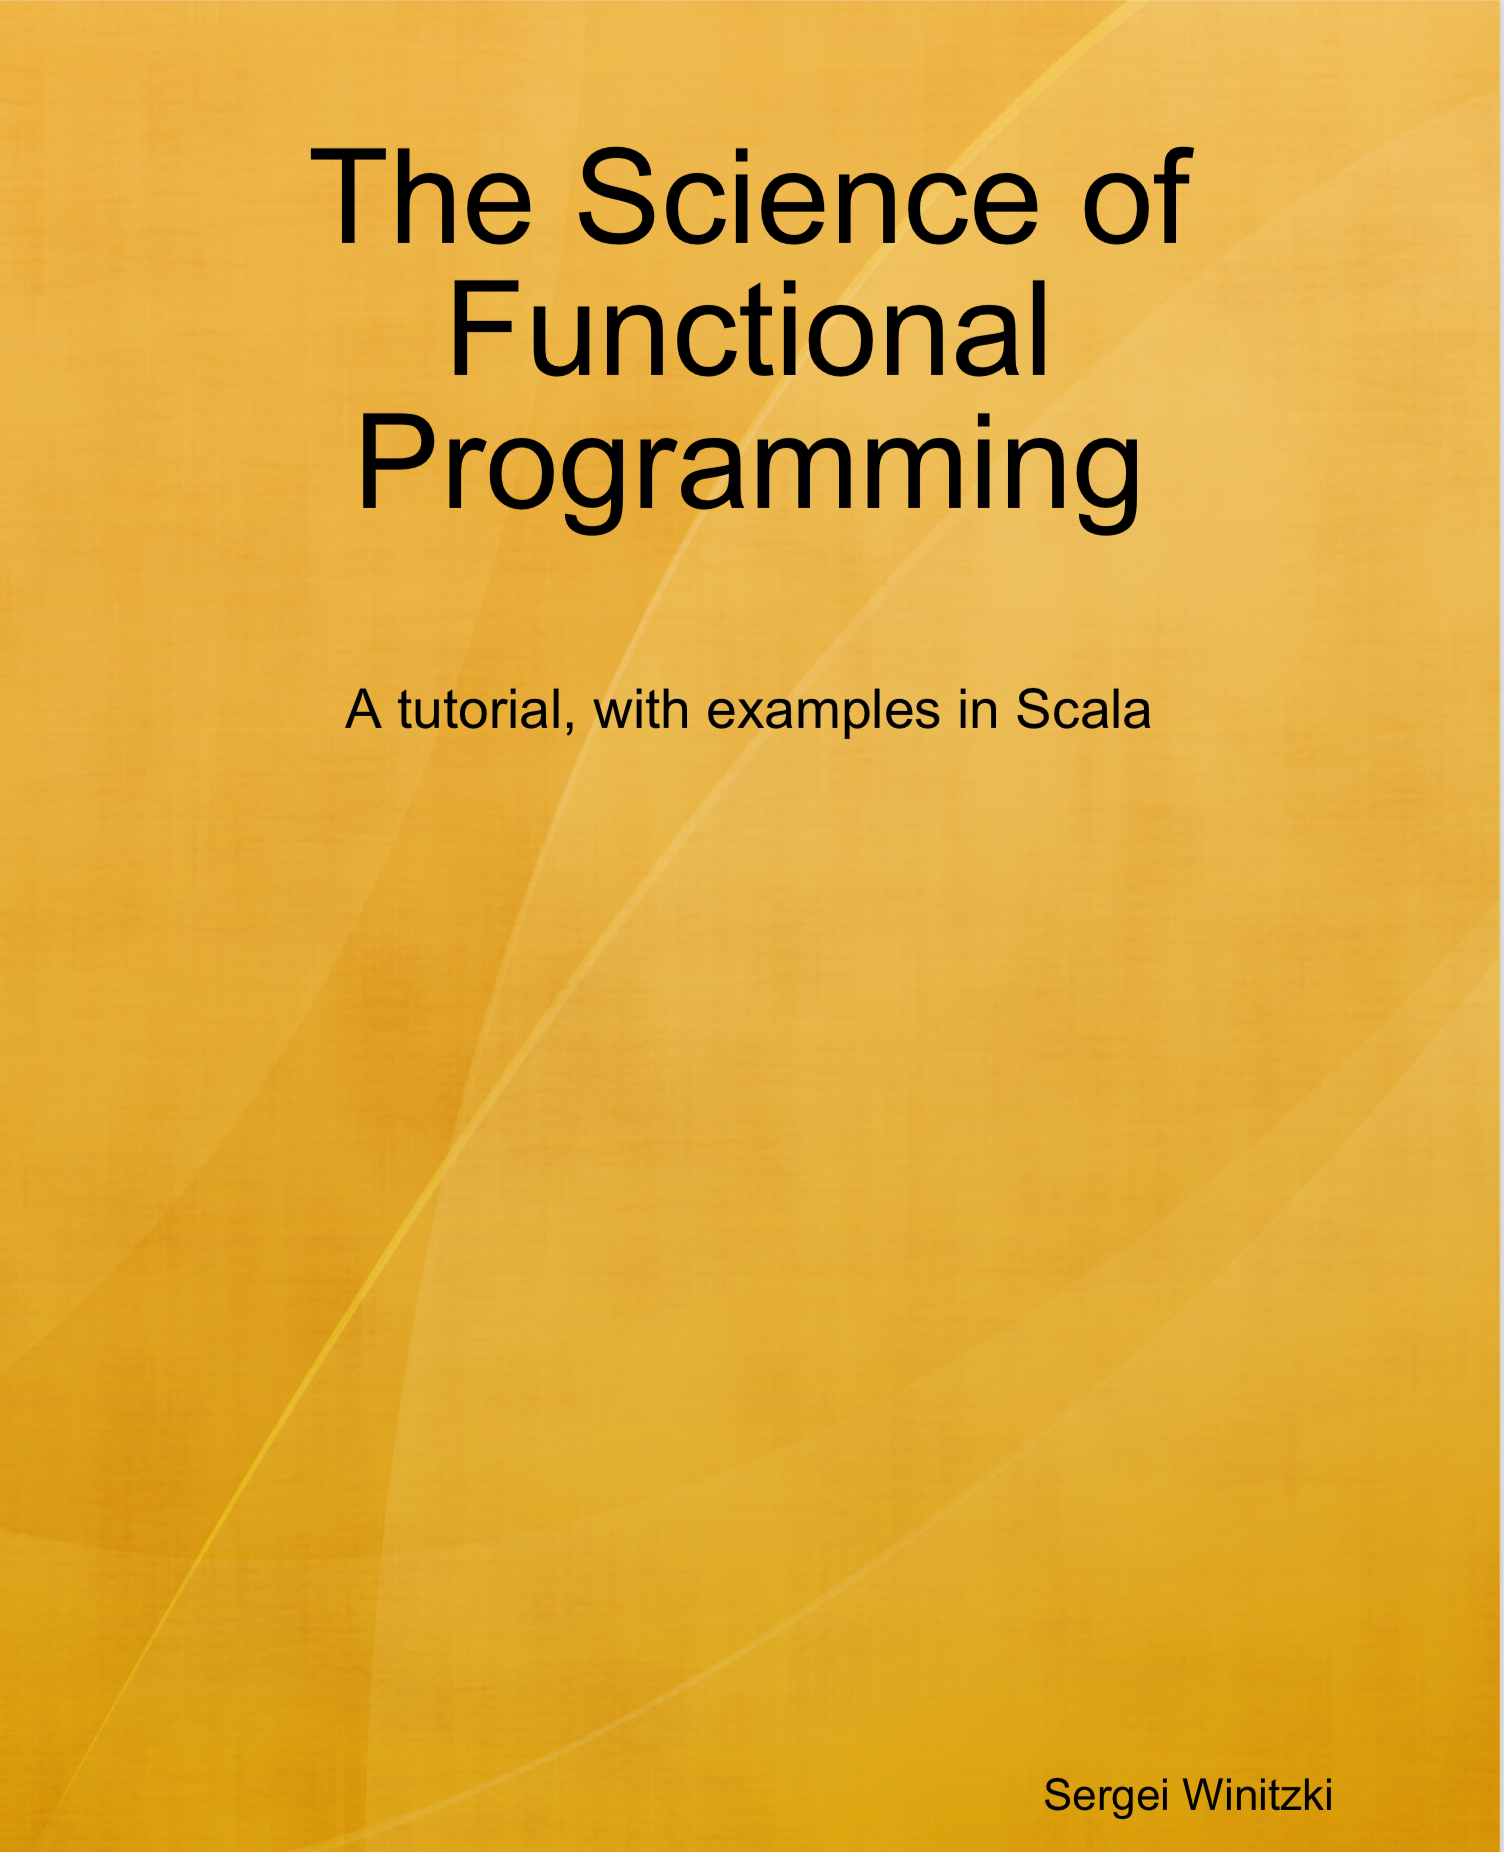
\includegraphics[width=2.5cm]{book-draft-cover}%
\end{minipage}{\small\par}
\par\end{center}

\end{frame}

\end{document}
